\documentclass{article}

\usepackage[russian]{babel}

\title{Лабораторная работа 3}
\author{Генералов Даниил, НПИ-01-21, 1032212280}

\usepackage[margin=10mm]{geometry}

\usepackage{listings}
\usepackage{graphicx}

\begin{document}
\maketitle

\section{Задание}

В системе передачи цифровой информации разговор передается в цифровом виде.
Речевые пакеты поступают через 6 ± 3 мс и передаются через два последовательно
соединенных канала. В каждый момент времени каждый из каналов может передавать
только один пакет. В случае занятости канала пакеты сохраняются в накопителях перед
каждым каналом. Время передачи пакета по каждому из каналов имеет экспоненциальное
распределение со средним значением 5 мс. Пакеты, время передачи которых больше 10 мс
(без учета времени ожидания), на выходе системы уничтожаются, поскольку длительное
время передачи значительно снижает качество передаваемой речи. Уничтожение свыше
30\% пакетов недопустимо. При достижении такого уровня система за счет ресурсов
ускоряет передачу в каналах до среднего значения времени 4 мс. При снижении уровня до
приемлемого значения происходит отключение ресурсов. Промоделировать 10 c работы
системы. Определить частоту уничтожения пакетов, частоту подключения ресурсов и
среднее время нахождения одного пакета в системе передачи информации (c учетом
времен ожидания).

\section{Код}

Ниже приведен код для решения этой задачи.
В этом коде создаются пакеты, которые проходят через два последовательных узла СМО.
Внутри каждого из узлов, после выхода из очереди, производится проверка, подключены ли ресурсы
(SAVEVALUE \texttt{turbomode}), и если да то смещается распределение времени обработки.
На выходе из системы проверяется время обработки пакета -- 
если оно в сумме больше 10мс, то увеличивается счетчик удаленных пакетов.
Затем выполняется решение, подключить или отключить ресурсы,
и решение подключить ресурсы когда они выключены записывается.

\lstdefinestyle{verbat}{
    basicstyle=\footnotesize\ttfamily,
    %xleftmargin=\parindent,
    frame=L,
}

\lstinputlisting[style=verbat]{lab3.gpss}

\section{Отчет}

Ниже приведен стандартный отчет GPSS World.
В нем показано, что за 10000мс через систему прошло 1676 пакетов, 
а удалено было 500 -- общий процент удаленных пакетов 29.8\%, что меньше 30\%.
Также в отчете приведены таблицы с распределением времени обработки пакета
и временем от начала до конца жизни пакета.
Эти таблицы также показаны ниже в виде картинок.
Из отчета также видно, что ресурсы подключались 102 раза за этот период,
то есть в среднем \textbf{раз в 98.03мc}.

Среднее время обработки пакета -- \textbf{8.937мс};
среднее время жизни пакета -- \textbf{14.505мс}.


\lstinputlisting[style=verbat]{lab3.report}

\newpage

Время обработки пакета:

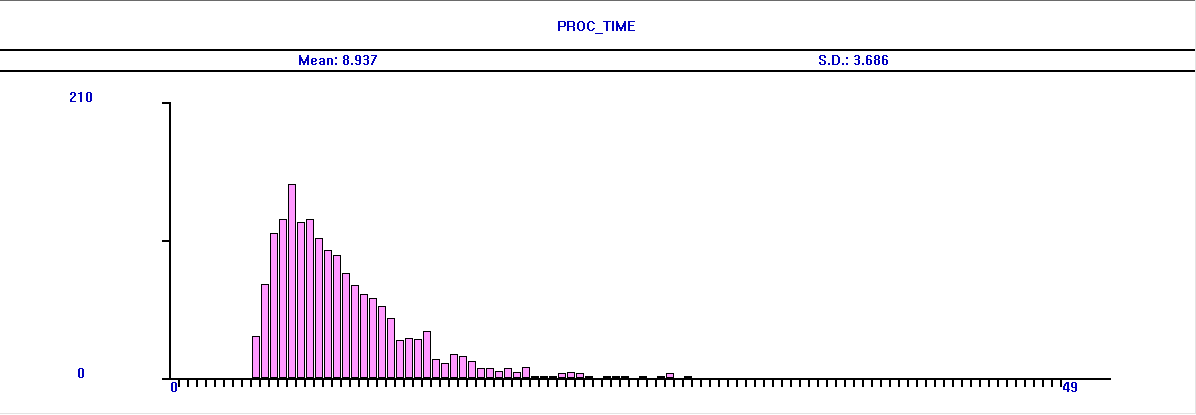
\includegraphics[width=\textwidth]{table2}

Время жизни пакета:

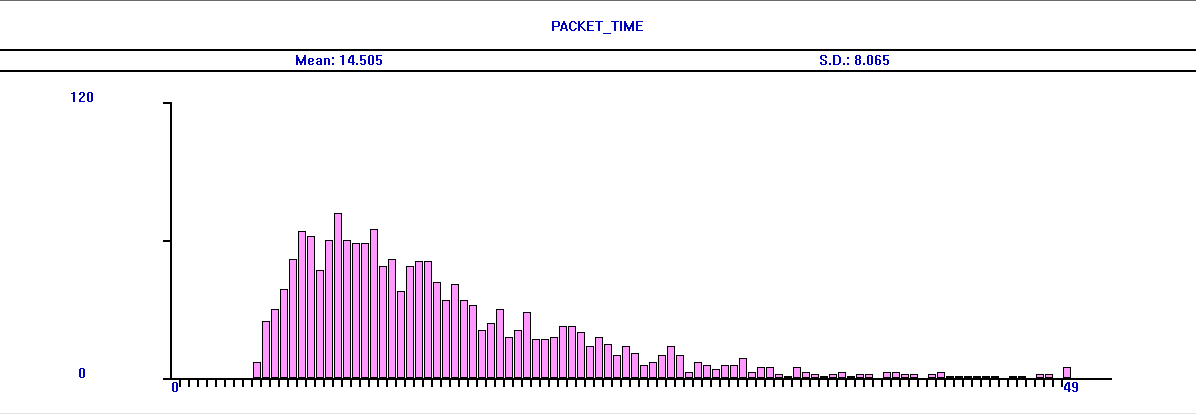
\includegraphics[width=\textwidth]{table1}


\end{document}